\section{Architecture and Design}
\label{section:architecture-and-design}

In this section we motivate and present the flavour of an approach for developing the architecture and design of a BX, including MDE languages that can be used to capture detailed designs of BX, as well as techniques for expressing and applying design patterns for BX. What we present here builds on the techniques introduced in the last section, where we used \transml\ to capture requirements for BX. We omit an end-to-end example, instead aiming to focus on touching on a variety of techniques that can be used to engineer BX solutions.

As discussed earlier, large and complicated BX are similar to large and complicated software systems: they involve many parts (e.g., transformation components, rules) with complicated inter-relationships and dependencies. Many BX have sophisticated behaviour which can be difficult to interpret from their concrete syntax. They are also difficult to engineer correctly. Large software systems are usually not monolithic: they are built as a set of interrelated components. Arguably, BX should be constructed in the same way. 

Nevertheless, architecture for BX -- and transformations in general -- can be complicated. Some of the issues are as follows.
\begin{itemize}
\item \textit{Components:} what are appropriate component models for BX? For software systems we have a reasonable understanding of what a component in a software architecture is, how it may be implemented, and how it can be precisely combined with other components. Our understanding of components for BX and transformations in general is underdeveloped. Most transformation languages offer a notion of a \textit{rule}, and some languages have a notion of \textit{module}, but richer and deeper understanding (e.g., of ports, protocols, and architectural styles) is missing.

\item \textit{Relationships:} what are appropriate relationships that can be defined between BX components? For software systems we have a comprehensive library of component connectors (e.g., protocols, buffers, compositions, containments) that can be deployed; a similar understanding for BX is not yet available.

\item \textit{Interoperability:} a key aspect of software architecture is what it provides in terms of interoperation with external systems. For BX, the question is: how can a BX be integrated with other components or architectures, e.g., code generators, verification tools, etc. 
\end{itemize}

We will now present an approach to transformation architecture embodied in \transml\  and present several small examples of both BX architecture and unidirectional transformation architecture. We then describe an approach for detailed design for transformations.

\subsection{BX Architecture in \transml\ }
In Section~\ref{section:requirements} we introduced the \transml\ approach and explained its support for requirements specification (including scenarios and formal requirement specification). As illustrated  in Figure~\ref{fig:transML}, \transml\ provides support for expressing transformation architectures and designs. 

Architecture in \transml\ is embodied in a traditional architectural modelling approach: an architecture is a set of components and connectors that interact via directional interfaces. Component types are given in terms of metamodels, or event types (for supporting event-driven architectures or for events generated by sensors) or other components (to support higher-order transformations). The component model is general in the sense that it can be used to represent transformations, black-box components (e.g., non-transformation or non-MDE components), or actors (e.g., human users). 

The \transml\ metamodel for architectures is illustrated in Figure~\ref{fig:transml-architecture}. It is worth noting the \textit{direction} attribute on the Interface element; components of BX may both generate and receive  information via interfaces.

\begin{figure}[htbp]
\centering{\scalebox{0.6}{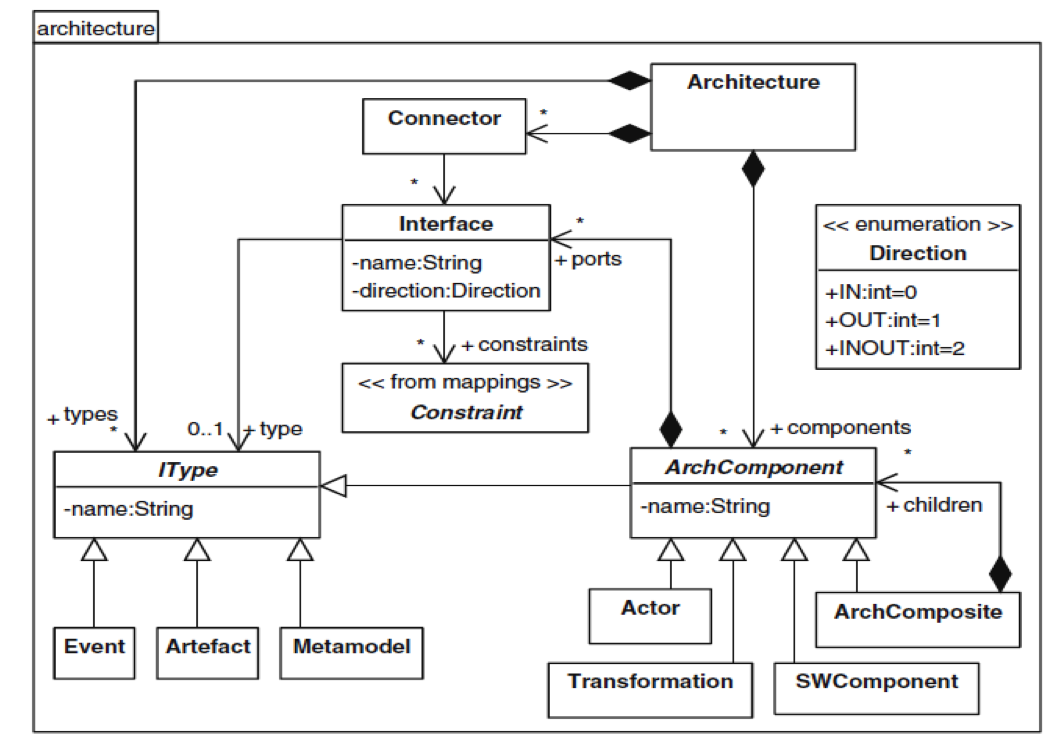
\includegraphics{transml-architecture.png}}}
\caption{\transml\ architecture metamode \cite{GuerraLKPS13}}
\label{fig:transml-architecture}
\end{figure}

Constraints on interfaces can be used to impose a concept of contract, e.g., to restrict expected inputs and outputs, but also to support conformance checking.

Figure~\ref{fig:architecture-example1} shows an example of a unidirectional transformation architecture, using a simple component-based concrete syntax from UML. This example illustrates a transformation-centric view, i.e., the components in the architecture are themselves transformations. This can be contrasted with a type-centric architecture, shown in Figure~\ref{fig:architecture-example2}, where the components are types (or metamodels). In both cases, the example architecture is for a chain of transformations between an object-oriented model and SQL code.

\begin{figure}[htbp]
\centering{\scalebox{0.6}{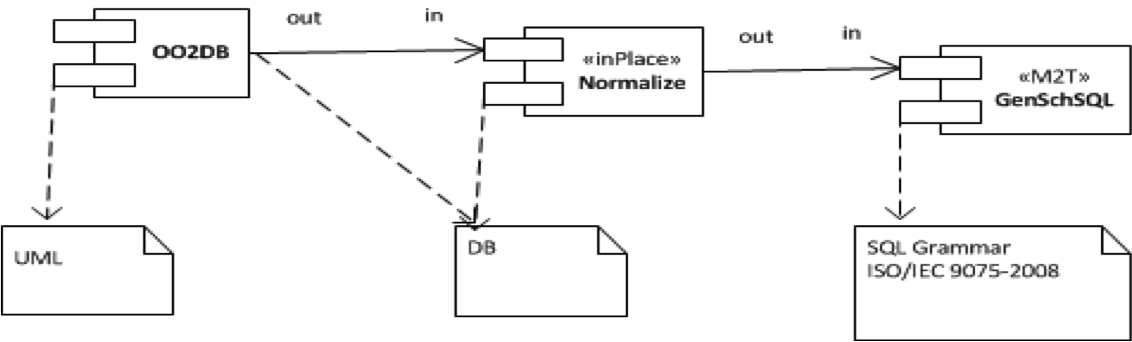
\includegraphics{transml-arch-example1.png}}}
\caption{\transml\ architecture example (transformation-centric, undirectional)}
\label{fig:architecture-example1}
\end{figure}

In the above example, firstly a unidirectional OO2DB transformation is executed (taking a UML model as input and producing a DB model as output). Then, a normalising update-in-place transformation is executed on the DB model. Finally, a model-to-text transformation is executed on the DB model, producing SQL code compliant to a specific grammar.

\begin{figure}[htbp]
\centering{\scalebox{0.4}{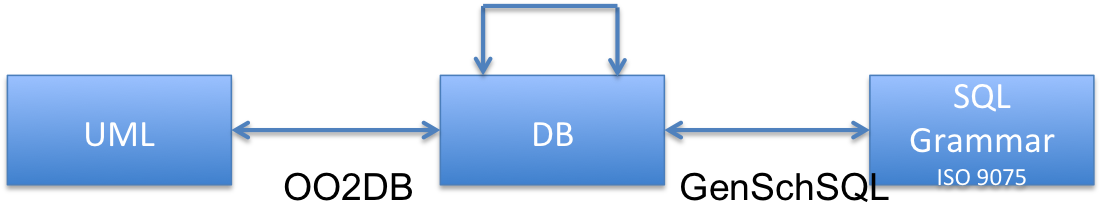
\includegraphics{transml-arch-example2.png}}}
\caption{\transml\ architecture example (type-centric, bidirectional)}
\label{fig:architecture-example2}
\end{figure}

The type-centric view represents the individual transformations as relationships between components. We have extended this example to represent bidirectional transformations throughout: i.e., OO2DB, Normalise and GenSchSQL (the model-to-text transformation) could be executed in either direction.  We could, of course, present the same BX in a transformation-centric style. In this case, the architecture in Figure~\ref{fig:architecture-example1} would have bidirectional dependencies on the relevant input and output models, as depicted 
in Figure~\ref{fig:architecture-example3} (in the figure we have circled the ports and connectors to highlight the bidirectionality of information flow).

\begin{figure}[htbp]
\centering{\scalebox{0.6}{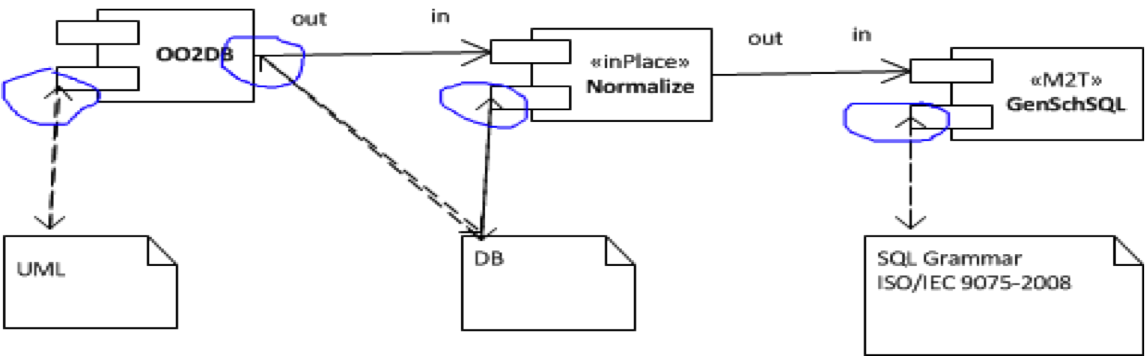
\includegraphics{transml-arch-example3.png}}}
\caption{\transml\ architecture example (transformation-centric, bidirectional)}
\label{fig:architecture-example3}
\end{figure}

\subsection{Design of BX}
The architecture of a software system captures the key components and their interrelationships. In the case of a BX this includes the connections between transformation components, the ports through which components communicate, and restrictions and constraints on that communication. The engineering process for BX continues with design, which can be broken into two parts: \textit{high-level design}, which focuses on capturing \textit{what is transformed into what}; and \textit{low-level design}, which focuses on capturing \textit{how} the transformation is to be carried out. We briefly consider \transml\ support for each aspect.

High-level design of a BX, once again, aims to capture what is transformed into what. To represent this, \transml\ introduces a \textit{mapping diagram}, inspired by triple graph grammars. These capture the mappings between arbitrary model elements involved in the transformation. However, mappings are not meant to be used as a implementation model -- specifically, they are not meant to be used as a tracing mechanism to guide the execution of code (this, as we will soon see, is the purpose of the low-level design features of the \transml\ family of languages).

The \transml\ metamodel for mapping diagrams is illustrated in Figure~\ref{fig:transml-mapping-diagram}. Mappings have ends which are associated with modelling elements. Navigability is a property of mappings; BX will involve navigation to both source and target. Constraints can be attached to mappings in order to define conditions on when (part of) a mapping can hold. 

\begin{figure}[htbp]
\centering{\scalebox{0.6}{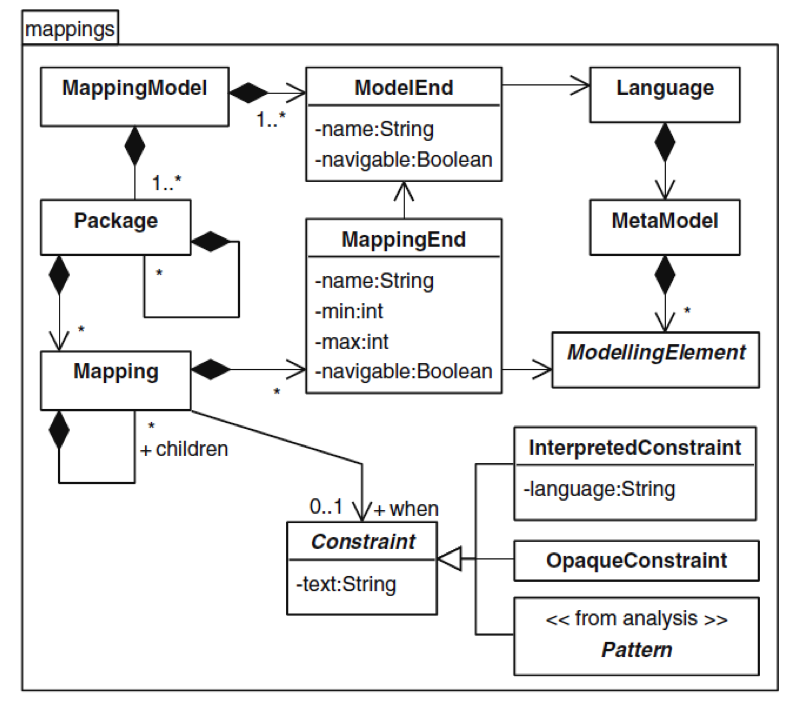
\includegraphics{transml-mapping-diagram.png}}}
\caption{\transml\ mapping diagram metamodel \cite{GuerraLKPS13}}
\label{fig:transml-mapping-diagram}
\end{figure}

Figure~\ref{fig:transml-mapping-example1} illustrates a mapping, for the OO2DBl BX. On the left of the diagram is a package containing key modelling elements of an OO model; on the right, a database model. In the centre are the mappings along with some informal English text explaining the purpose of each distinct mapping. Note the navigability of each rule; these can be executed from a DB model to an OO model, or vice versa.

\begin{figure}[htbp]
\centering{\scalebox{0.5}{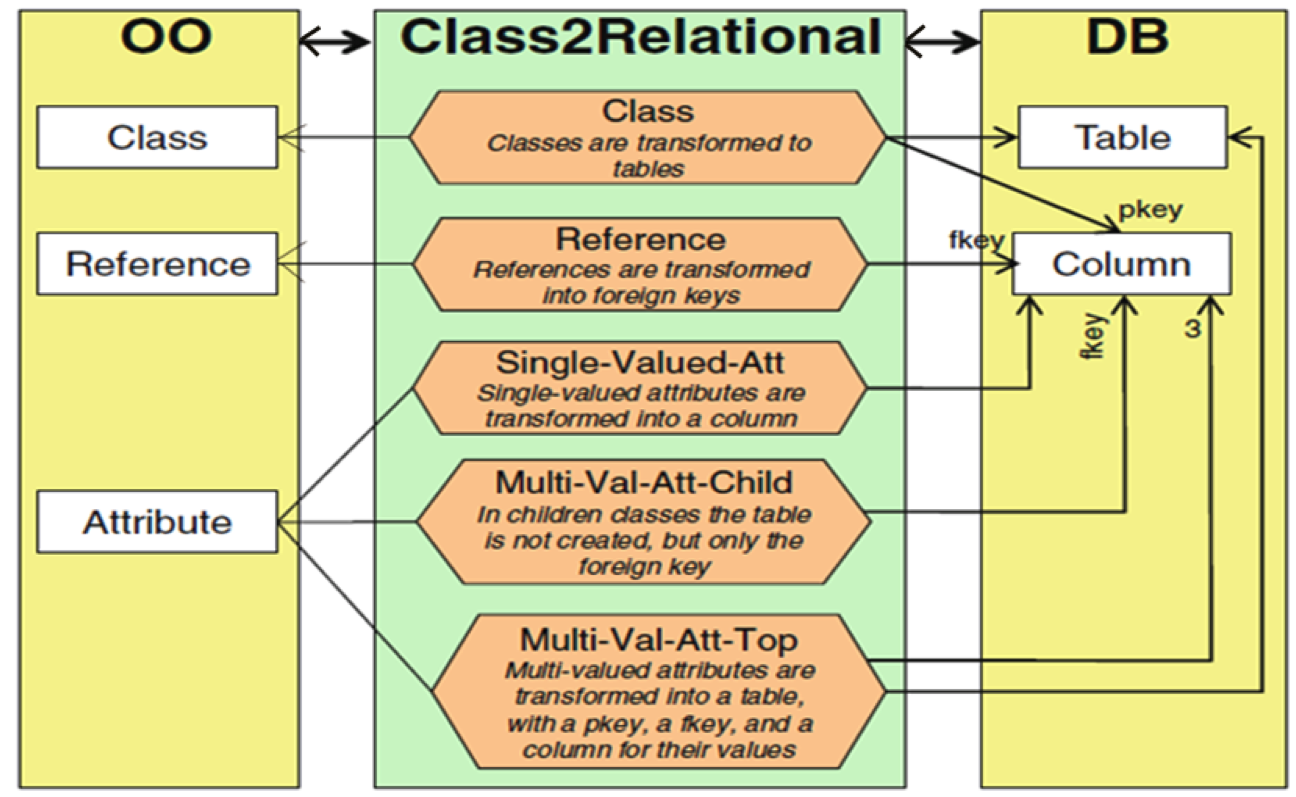
\includegraphics{transml-mapping-example1.png}}}
\caption{\transml\ mapping example \cite{GuerraLKPS13}}
\label{fig:transml-mapping-example1}
\end{figure}

The next example, in Figure~\ref{fig:mapping-example3}, elaborates what is presented in Figure~\ref{fig:transml-mapping-example1} and imposes a constraint on the very last mapping, Multi-Val-Att-Top. The constraint, expressed in OCL, states that the owner of an attribute cannot have any parent classes; this is so that multi-valued attributes can be appropriately flattened into a table.

\begin{figure}[htbp]
\centering{\scalebox{0.5}{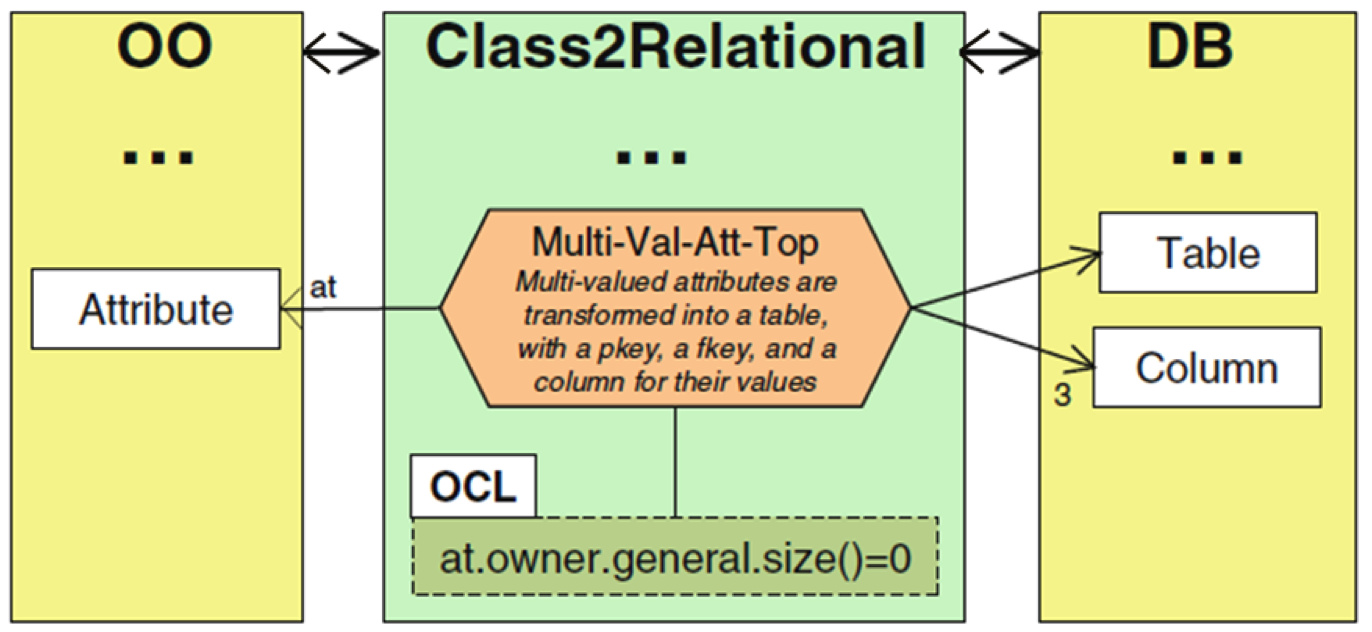
\includegraphics{transml-mapping-example2.png}}}
\caption{\transml\ mapping example (constraint) \cite{GuerraLKPS13}}
\label{fig:mapping-example3}
\end{figure}

While high-level design is supported in \transml\ via mapping diagrams, low-level design -- which is where the transition to implementation begins -- is
supported by more detailed diagrams. Technically, low-level design \textit{could} be supported by using a favourite BX programming language. But it may be preferable -- for reasons of process -- to maintain a degree of platform independence while still focusing on the essential aspects of BX development. As such, \transml\ provides low-level design languages for capturing the \textit{structure} of BX rules, control flow, and blocks. These are encapsulated in two diagrams: the \textit{rule structure diagram} and the \textit{rule behaviour diagram}.

The rule structure diagram (metamodel in Figure~\ref{fig:transml-rulestructure}) is used to refine a mapping diagram. A rule in such a diagram can contribute to the implementation of one or more mappings. Rules themselves may be unidirectional or bidirectional. Structure diagrams also allow for explicit or implicit (e.g., nondeterministic) capture of execution flow, via subclasses of the \textit{Flow} metaclass. In particular, a set of rules can be placed inside a nondeterministic block, for example, as in graph transformation programs.

\begin{figure}[htbp]
\centering{\scalebox{0.5}{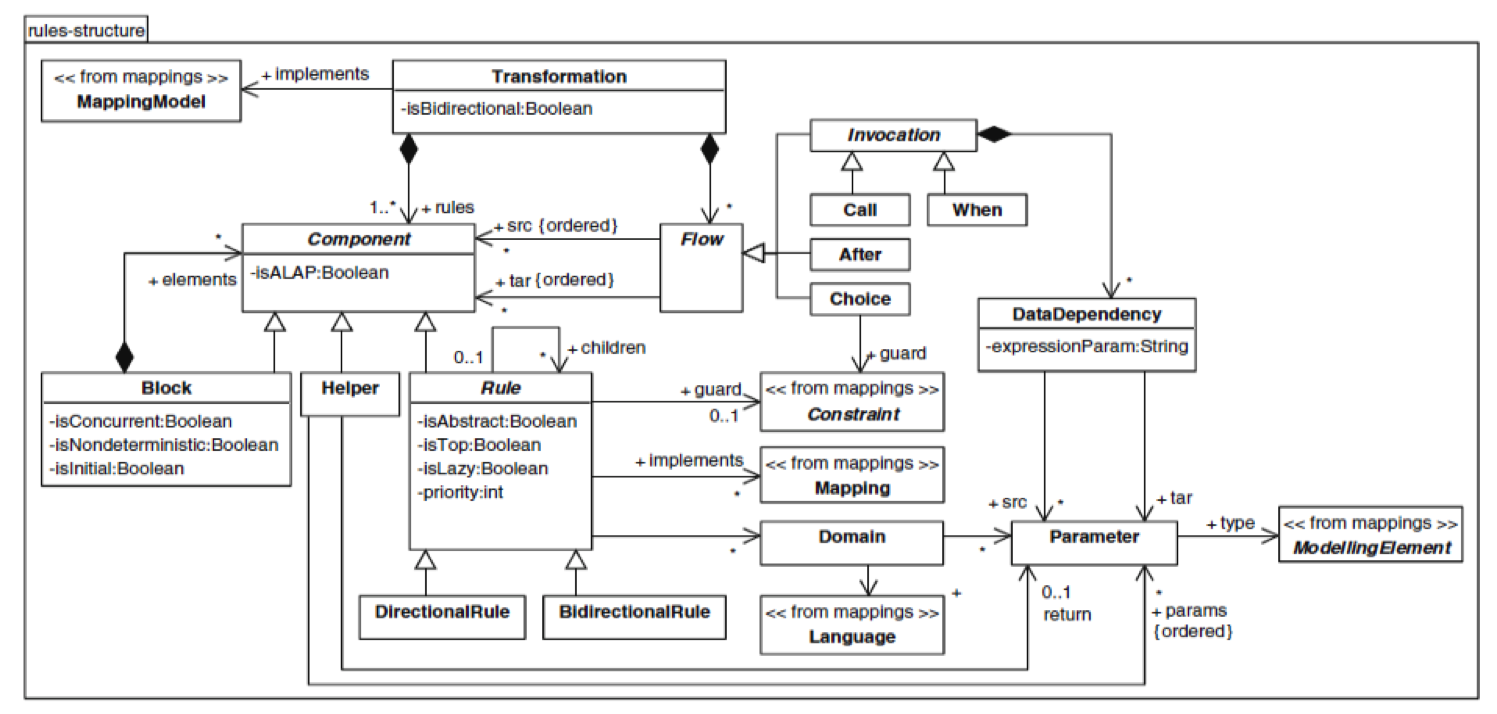
\includegraphics{transml-rulestructure-diagram.png}}}
\caption{\transml\ rule structure diagram metamodel \cite{GuerraLKPS13}}
\label{fig:transml-rulestructure}
\end{figure}

Effectively, rule structure diagrams capture the structure rules, execution flow and data dependencies. This is illustrated in Figure~\ref{fig:transml-rulestructure-example}, which shows a directional transformation from an object-oriented model to a database model. The structure in particular is tailored to a representation of rules in the Epsilon Transformation Language (ETL). There is a top-level rule (Class2Table) that is executed initially; its execution is followed by a block of rules that execute nondeterministically; these populate the structure of a database table (i.e., Reference2Column, SingleValuedAtt2Column, MultiValuedAtt2Table). Note that blocks can be a useful mechanism for design, even if the ultimate implementation language does not support them (for example, ETL does not support blocks directly).

\begin{figure}[htbp]
\centering{\scalebox{0.6}{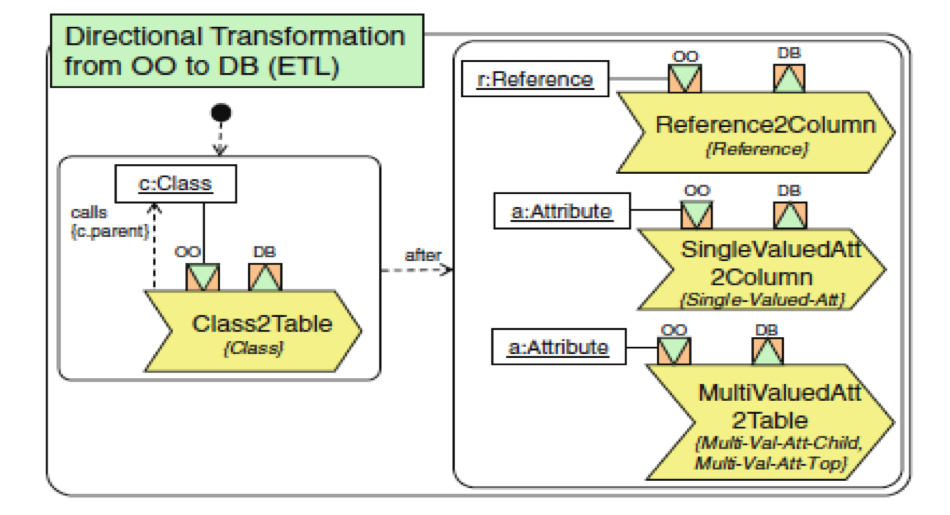
\includegraphics{transml-rulestructure-example.png}}}
\caption{\transml\ rule structure diagram example \cite{GuerraLKPS13}}
\label{fig:transml-rulestructure-example}
\end{figure}

A second example is shown in Listing~\ref{listing:bx-blocks}. In this case, a small domain-specific BX language is used to specify parts of a transformation between trees and graphs. The transformation is divided into two nondeterministic blocks; these blocks encapsulate bidirectional rules between elements of one model (e.g., Tree) and elements of a second model (e.g., Node). 

\begin{lstlisting}[float,floatplacement=H,basicstyle=\ttfamily,caption=An example of a BX using blocks, captionpos=b, label=listing:bx-blocks]
transformation Tree2Graph {
  nondeterministic RuleBlockForward {
     bidirectional Tree2Node { ... };
     bidirectional TreeEdge2GraphEdge {...};
   }
   
   nondeterministic RuleBlockBackward {
      bidirectional TreeLabelsfromNodeLabels {...};
      bidirectional TreeEdgesfromGraphEdges { ... };
    }
}
\end{lstlisting}
Rule structure diagrams in particular need to take into account the choice of ultimate implementation language. This is because these diagrams capture execution flow, which is platform specific. For example, consider ETL: the execution flow model is such that each rule is executed once at each instance of input; by comparison, in a graph transformation language, execution is for ``as long as possible'', i.e., until a fix-point is reached. As such, a specific rule structure diagram may be transformed easily to one implementation language, but not another. The metamodel for rule structures is, in our experience, sufficiently generic to capture a number of transformation implementation languages, but there may be specific features of specific implementation languages that we have not considered that are not easily supported.

The rule structure diagram treats rules as black boxes, ignoring their behaviour. As such, concepts such as attribute contribution, object creation, or link configuration will be ignored. These can all be specified using implementation languages such as ETL, but \transml\ also provides a diagram for their specification: the rule behaviour diagram. This allows the behaviour of rules to be captured using an action language, or declarative graphical pre- and postconditions, or object diagrams annotated with operations (similar in a sense to Catalysis snapshots). An example unidirectional rule behaviour diagram is shown in Figure~\ref{fig:transml-rule-behaviour-example}. On the left of the figure is a snapshot with annotations indicating creation of objects. On the right is the ETL program that would correspond to such a diagram.

 \begin{figure}[htbp]
\centering{\scalebox{0.6}{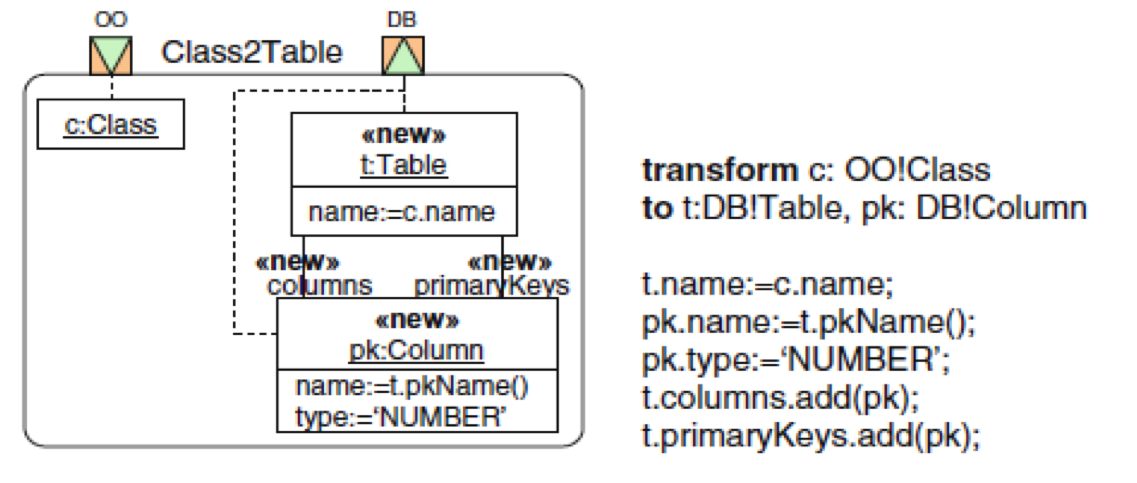
\includegraphics{transml-rulebehaviour-example.png}}}
\caption{\transml\ rule behaviour diagram example \cite{GuerraLKPS13}}
\label{fig:transml-rule-behaviour-example}
\end{figure}

It should be noted that while we have broad and quite deep experience of using \transml\ for engineering unidirectional transformations, we have much less experience of using it for engineering BX. Using some of the features of \transml\ for capturing different aspects of BX may be a useful contribution to the BX community, as they provide platform-independent ways of specifying different features.

\subsection{Design Patterns for BX}
In this section we very briefly discuss several design patterns \cite{Gof1995} for BX. Design patterns in general capture recurring design problems (e.g., in object-oriented design) and their solutions. Solutions generally need to be instantiated for particular problem concepts. Many different patterns have been developed and captured in the literature, including some for model transformations. In this section we present three examples, taken from Lano et al \cite{LanoKR14} with some customisation for our context.

\subsubsection{Auxiliary Correspondence Model Pattern}
A special kind of model transformation is a \textit{merging} or \textit{weaving}, where two or more models are combined into a single model. This weaving process can be carried out in batch mode or via a change propagation approach, where changes from the models being combined can be propagated to others. In doing so, most such transformations make use of a so-called \textit{auxiliary correspondence model}. This is a design pattern: the auxiliary correspondence model defines auxiliary model elements and associations that link source and target elements. It can be used to record mappings performed by a BX and to propagate modifications when one model changes. The benefit of using such a pattern is that it separates concerns: the source and target models are kept separate from the connections that link their elements. In turn, these explicit links between source and target model can make it easier to check correctness and coverage in the transformation. The disadvantage of applying this pattern is that it requires maintenance of an additional model.

\subsubsection{Unique Instantiation Pattern}
This pattern focuses on improving the efficiency of transformations. In particular, it is applied to avoid duplicating model elements in either the source or the target of a BX. In particular, the pattern imposes a check that an element satisfying specified properties does not exist, before the element is actually created in the source or target. For example, in a QVT-Relations transformation that has applied this pattern, new elements will not be created if there are already elements that satisfy the relations specified; this is really at the heart of check-before-enforce mode in QVT-Relations. The benefit of using this pattern is that it can help ensure hippocraticness; the disadvantage is the test for existence, which can degrade BX performance. However, we note that other patterns, e.g., related to indexing \cite{LanoKR14} -- and model indexing frameworks like Hawk -- can help offset this.

\subsubsection{Map Objects Before Links Pattern}
This pattern is used to separate the relation between elements in source and target models from the relations between \textit{links} in the models. A particular application of this pattern would be to structure a transformation wherein model elements are transformed before the relations between model elements (i.e., nodes before edges). Such an execution flow may be useful in cases where models may have self-associations or circular dependencies. The benefit of using this pattern is similar to that of the Visitor pattern \cite{Gof1995} in object-oriented design: the specification of the transformation is modular and processing for a new type of association in a modelling language can be more easily handled. The disadvantage of using this pattern is that while edges (relations) are treated modularly, nodes (model elements) may not be, and if a new feature is added to a language, it may require significant restructuring to the transformation that has used this pattern.

\subsection{Summary}
In this section we have discussed different aspects of the architecture and design of BX, covering abstract architecture for transformations, through high-level and low-level design, including behaviour of individual transformation rules, as well as a selection of design patterns that can be used to help increase cohesion and decrease coupling in our BX. We will next briefly discuss an approach to verification of BX, focusing on use of mathematical techniques.